\documentclass{article}


% if you need to pass options to natbib, use, e.g.:
%     \PassOptionsToPackage{numbers, compress}{natbib}
% before loading neurips_2022


% ready for submission
\usepackage{neurips_2022}


% to compile a preprint version, e.g., for submission to arXiv, add add the
% [preprint] option:
%     \usepackage[preprint]{neurips_2022}


% to compile a camera-ready version, add the [final] option, e.g.:
%     \usepackage[final]{neurips_2022}


% to avoid loading the natbib package, add option nonatbib:
%    \usepackage[nonatbib]{neurips_2022}


\usepackage[utf8]{inputenc} % allow utf-8 input
\usepackage[T1]{fontenc}    % use 8-bit T1 fonts
\usepackage{hyperref}       % hyperlinks
\usepackage{url}            % simple URL typesetting
\usepackage{booktabs}       % professional-quality tables
\usepackage{amsfonts}       % blackboard math symbols
\usepackage{nicefrac}       % compact symbols for 1/2, etc.
\usepackage{microtype}      % microtypography
\usepackage{xcolor}         % colors

\usepackage{enumitem}
\usepackage{graphicx}


\title{Algorithms for Searching the Initial Conditions of a Cosmology - Research Log}

% The \author macro works with any number of authors. There are two commands
% used to separate the names and addresses of multiple authors: \And and \AND.
%
% Using \And between authors leaves it to LaTeX to determine where to break the
% lines. Using \AND forces a line break at that point. So, if LaTeX puts 3 of 4
% authors names on the first line, and the last on the second line, try using
% \AND instead of \And before the third author name.


\author{%
  Albert Liang
  % examples of more authors
  % \And
  % Coauthor \\
  % Affiliation \\
  % Address \\
  % \texttt{email} \\
  % \AND
  % Coauthor \\
  % Affiliation \\
  % Address \\
  % \texttt{email} \\
  % \And
  % Coauthor \\
  % Affiliation \\
  % Address \\
  % \texttt{email} \\
  % \And
  % Coauthor \\
  % Affiliation \\
  % Address \\
  % \texttt{email} \\
}


\begin{document}


\maketitle


\begin{abstract}
    This is a personal research log to track the progress of the initial condition search project.
\end{abstract}

\section{Background}

In \cite{emulator}, the authors proposed a CNN model (i.e. the forward model, whose code can found in \href{https://github.com/thisisalbertliang/map2map/blob/search/map2map/models/styled_vnet.py#L8}{StyleVNet.py}) that emulates the evolution of a system of N-body particles interacting under the influence of Newtonian gravity on an expanding cosmological background, which is specified by 5 cosmological parameters $\mathcal{P} = \{ \Omega_m, \Omega_b, \sigma_8, n_s, h \}$. In particular, the forward model takes the linear, also known as the Zel'dovich approximiation (ZA), displacement field at redshift $z = 0$ and the values of $\mathcal{P}$ as inputs and outputs the nonlinear displacement fields also at redshift $z = 0$. The forward model effectively nonlinearizes the linear inputs, directly approximating the outcome of an N-body simulation by learning the mode couplings of the dark matter field.

The authors trained the forward model on 2000 simulations (red shift $z = 0$ snapshots) from the Quijote latin hypercube N-body suite \cite{quijote}. Each simulation has a unique set of 5 cosmological parameters $\mathcal{P}$, which were randomly sampled in a five dimensional latin hypercube. The simulation were run using the N-body code Gadget-3 \cite{gadget-3} with $512^3$ particles in a 1 Gpc $h^{-1}$ box.

The results showed that the forward model gives accurate results down to scales of $k \sim 1 Mpc^{-1} h$, which is a considerable improvement over prior works (e.g. COLA \cite{cola}).

However, although the forward model is successful in predicting the nonlinear displacement field for a given linear displacement field (i.e. ZA), the inference of the linear field for a given nonlinear displacement field (i.e. the backward direction) is still an unsolved problem.

\section{Problem}

We are interested in developing algorithms to infer/predict the linear/ZA displacement field (which is equivalent to the initial conditions of the cosmology up to constant scaling) given its corresponding nonlinear displacement field.

In particular, the inputs and outputs of our algorithm is
\begin{itemize}
\setlength\itemsep{-1em}
    \item \textbf{Input 1}: A ground truth nonlinear displacement field for an unknown linear displacement field. \\
    \item \textbf{Input 2}: The five cosmological parameters. \\
    \item \textbf{Output}: The inferred/predicted linear displacement field.
\end{itemize}

\section{Idea \#1: Gradient Descent}

Since the forward model appears to be a reliable emulator of the N-body evolution, one potential way to find the linear displacement field for a given nonlinear displacement field is to run \textbf{gradient descent} on the linear displacement field itself, fixing the forward model weights.

In particular, we would assume that we already have access to a pretrained forward model. We would initialize a field and then repeatedly run gradient descent on this field by back-propgating from the error between its predicted nonlinear displacement field (according to the forward model) and the given ground truth nonlinear displacement field.

There are several hyper-parameters/modeling choices that we need to address here:
\begin{enumerate}
\setlength\itemsep{-1em}
    \item How to define the error between the ground truth and predicted nonlinear displacement fields? (i.e. what should be our loss function?). \\
    \item How do we initialize the linear field? (can we just arbitrarily start from a known linear displacement field in the Quijote simulation data?) \\
    \item What optimizer should we use? (e.g. SGD? AdamW? )\\
    \item What learning rate should we use?
\end{enumerate}

\subsection{Some results}

To test this idea, I pre-trained a forward model on a single cosmology (I used the \texttt{LH0000} cosmology in Quijote) for 50 epochs. Then, I implemented and ran the aforementioned gradient descent idea on the following inputs:
\begin{itemize}
\setlength\itemsep{-1em}
    \item \textbf{Input 1}: A $40 \times 40 \times 40$ patch of the ground truth nonlinear displacement field from the \texttt{LH00045} cosmology in the Quijote dataset. (I couldn't load the whole $512 \times 512 \times 512$ field becuase our GPUs are too small) \\
    \item \textbf{Input 2}: The five cosmological parameters of the \texttt{LH0045} cosmology, of course.
\end{itemize}
where the hyper-parameters/modeling choices are set as follows:
\begin{enumerate}
\setlength\itemsep{-1em}
    \item $\mbox{loss}(\hat{Y}, Y) = \log \left( \mbox{MSE} \left( \mbox{Lagrangian}(\hat{Y}), \mbox{Lagrangian}(Y) \right)^3 \cdot \mbox{MSE} \left( \mbox{Eulerian}(\hat{Y}), \mbox{Eulerian}(Y) \right) \right)$ where $\hat{Y}$ and $Y$ are the predicted and ground truth nonlinear displacement fields respectively. This is the same loss function that was used in Drew's paper \cite{emulator}. \\
    \item I initialize the input field to a $40 \times 40 \times 40$ patch of the ground truth linear field from the same cosmology (i.e. the \texttt{LH0045} cosmology) that is \textbf{far away from} the indices of the previous $40 \times 40 \times 40$ patch from the ground truth nonlinear field. This initial input linear field is displayed in the \texttt{in} column of Figure \ref{fig:init-slices} \\
    \item I set the optimizer to the vanilla SGD. \\
    \item I set the learning rate to 100 (notice how large the learning rate is. I found that small learning rates like $0.001$ makes the training overly slow)
\end{enumerate}

Ideally, we hope the input linear field can converge to the ground truth linear field (displayed in the \texttt{true\_in} column of Figure \ref{fig:init-slices})

After running gradient descent for ~24 hours, I plotted the loss curves, the power spectrums, and slices of the displacement fields (shown in the next few pages)
% \begin{figure}
%     \centering
%     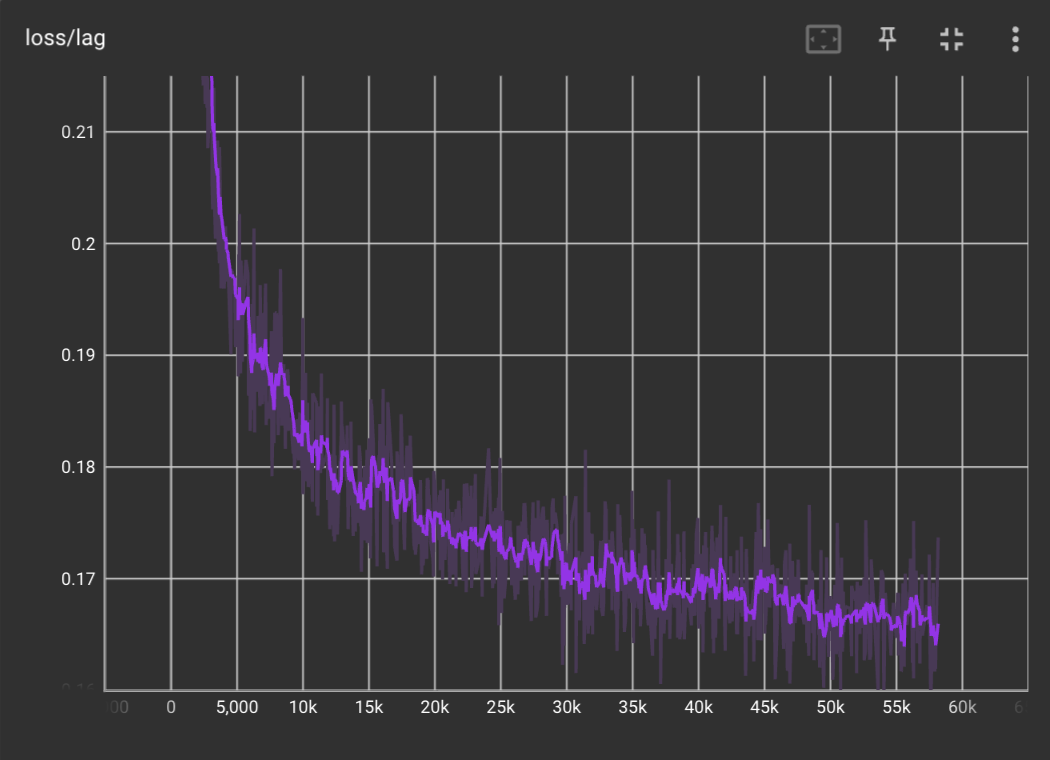
\includegraphics[width=10cm]{figs/lag-loss.png}\hfill
%     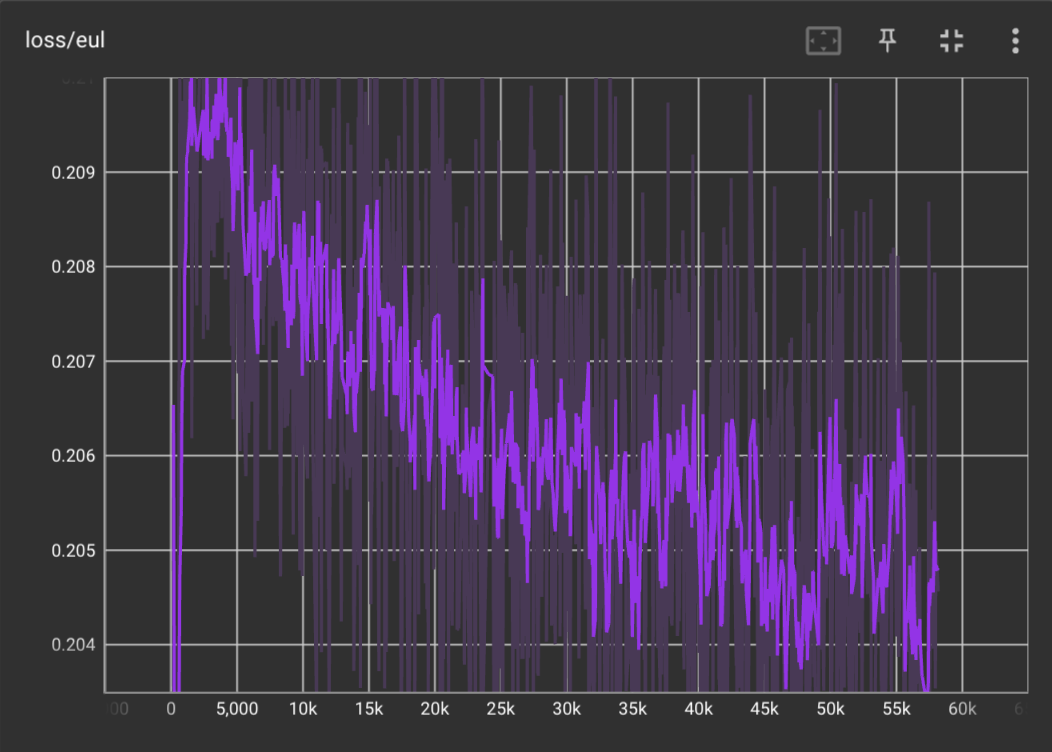
\includegraphics[width=10cm]{figs/eul-loss.png}\hfill
%     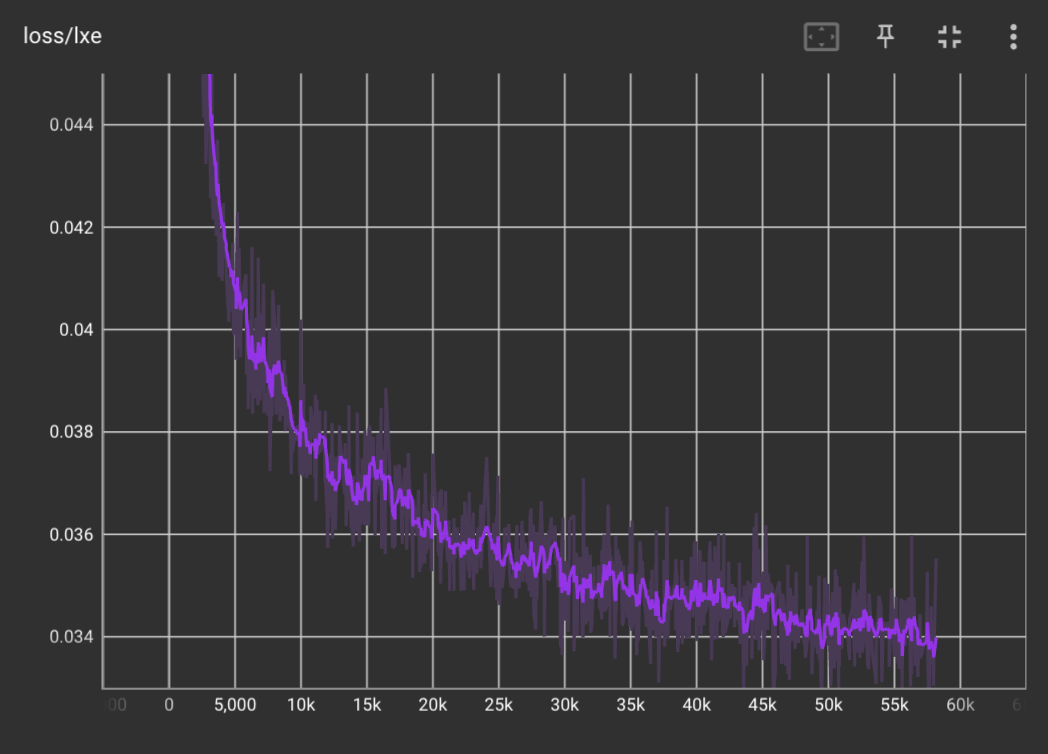
\includegraphics[width=10cm]{figs/lxe-loss.png}
%     \caption{Caption}
%     \label{fig:my_label}
% \end{figure}

\begin{figure}[h]
    \centering
    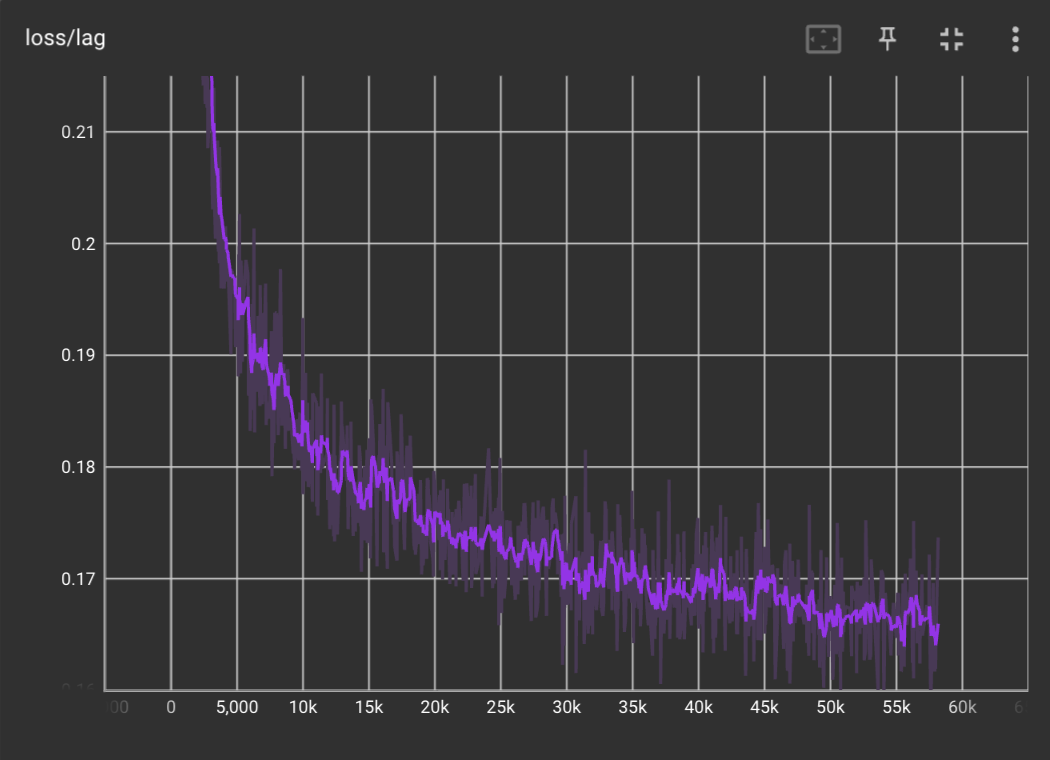
\includegraphics[width=10cm]{figs/lag-loss.png}
    \caption{Loss curve of $\mbox{MSE} \left( \mbox{Lagrangian}(\hat{Y}), \mbox{Lagrangian}(Y) \right)$}
    \label{fig:lag-lass}
\end{figure}

\begin{figure}[h]
    \centering
    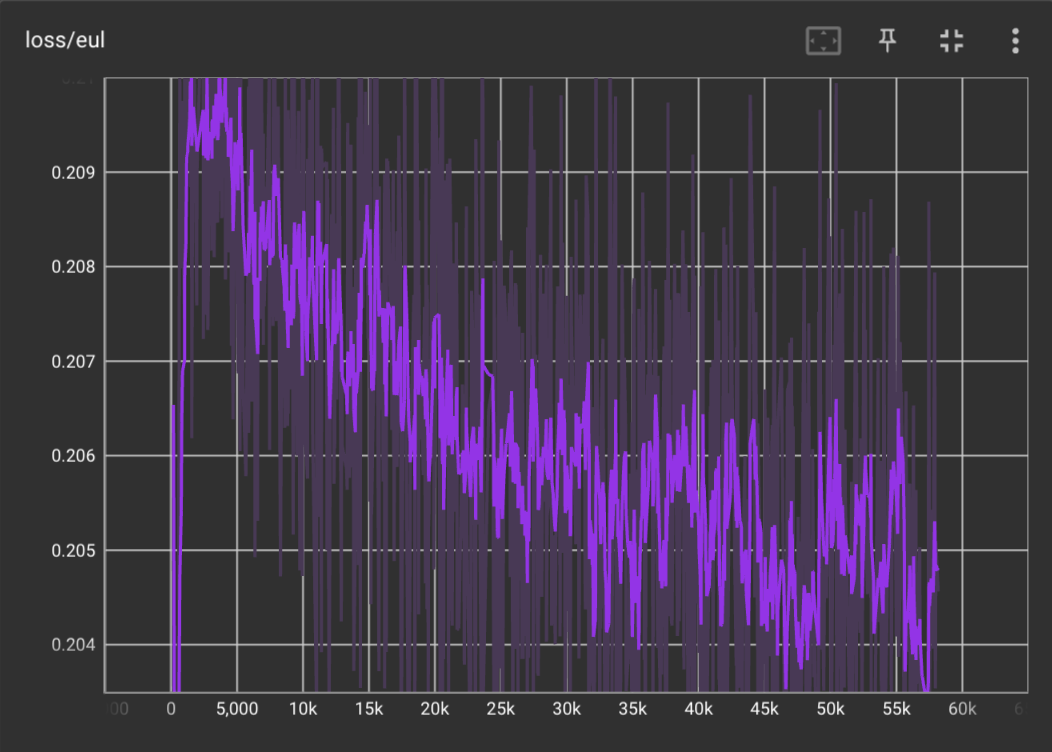
\includegraphics[width=10cm]{figs/eul-loss.png}
    \caption{Loss curve of $\mbox{MSE} \left( \mbox{Eulerian}(\hat{Y}), \mbox{Eulerian}(Y) \right)$}
    \label{fig:eul-loss}
\end{figure}

\begin{figure}[h]
    \centering
    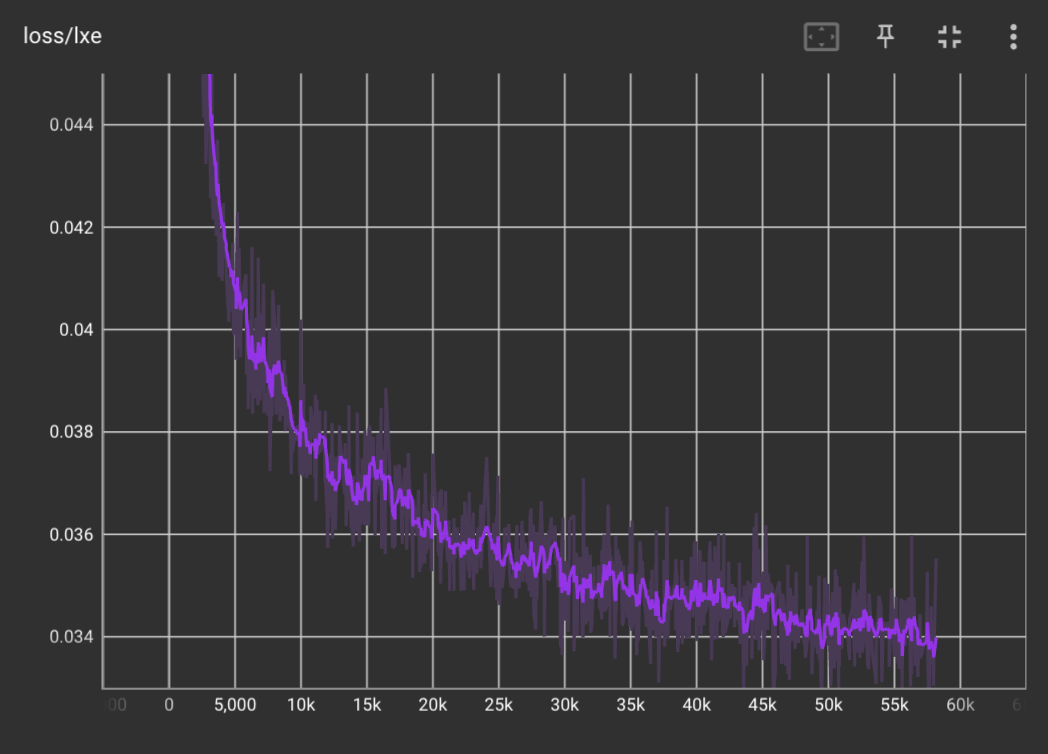
\includegraphics[width=10cm]{figs/lxe-loss.png}
    \caption{Loss curve of $\mbox{MSE} \left( \mbox{Lagrangian}(\hat{Y}), \mbox{Lagrangian}(Y) \right) \cdot \mbox{MSE} \left( \mbox{Eulerian}(\hat{Y}), \mbox{Eulerian}(Y) \right)$, i.e. their product}
    \label{fig:lxe-loss}
\end{figure}

\begin{figure}[h]
    \centering
    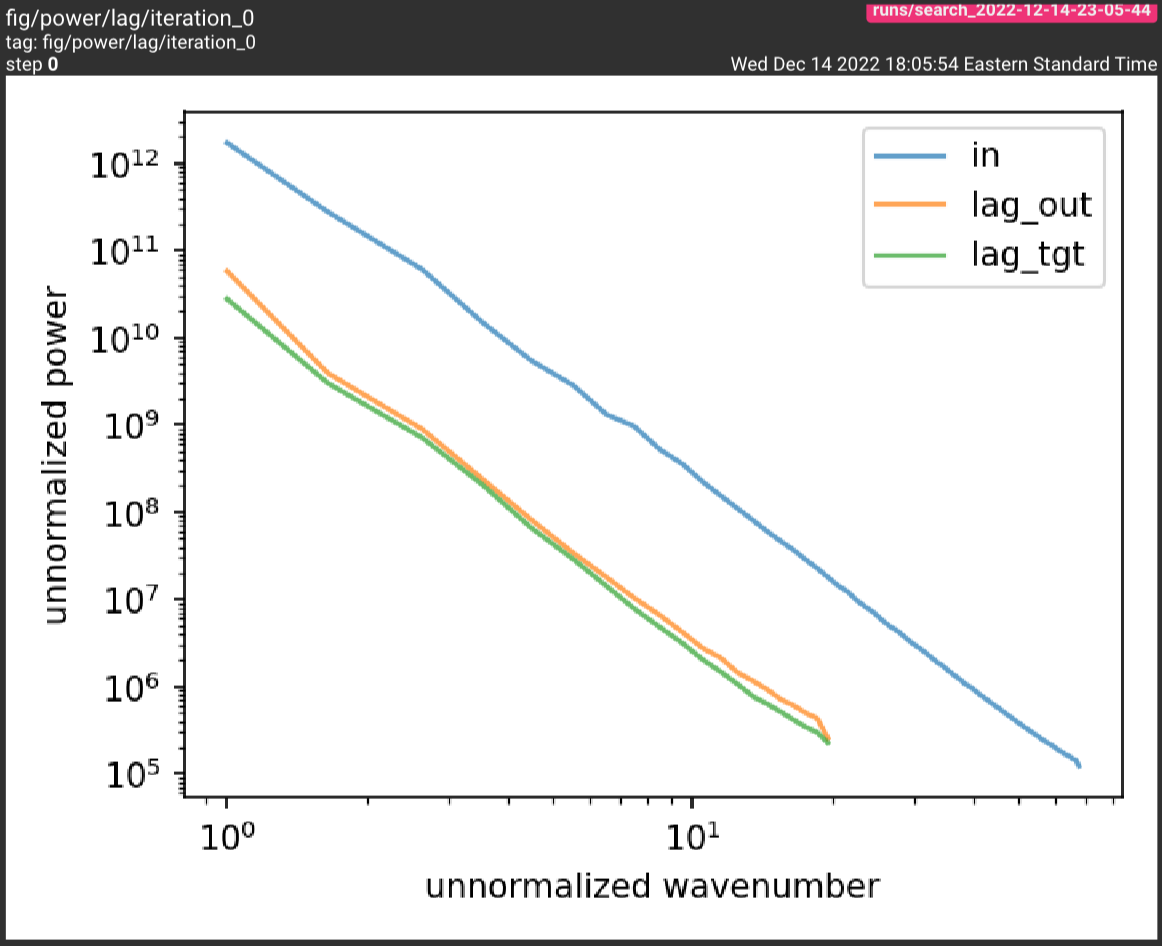
\includegraphics[width=10cm]{figs/initial-lag-pow-spec.png}
    \caption{This shows the Lagrangian power spectrum for the input at step 0 (i.e. the initial input that was initialized to a patch of the ground truth linear displacement field)}
    \label{fig:init-lag-pow}
\end{figure}

\begin{figure}[h]
    \centering
    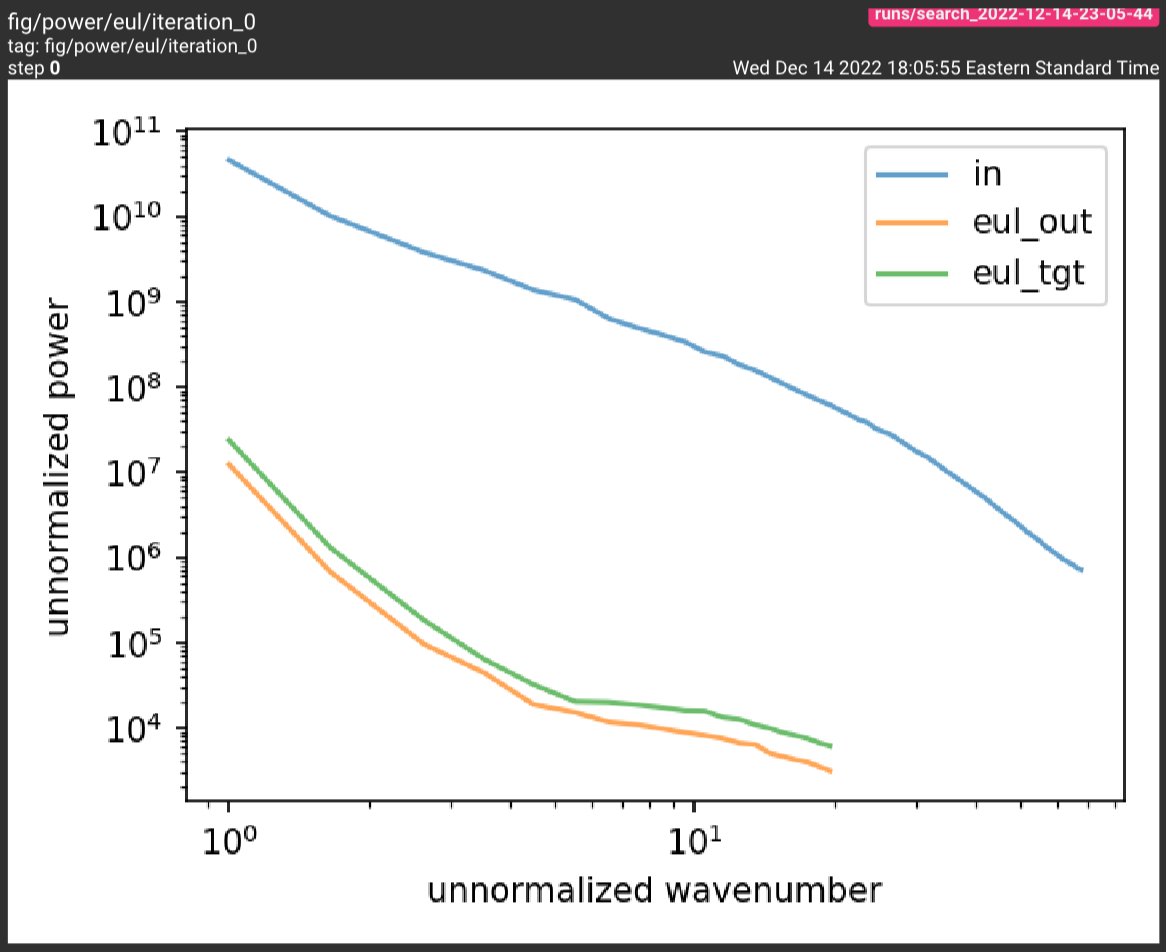
\includegraphics[width=10cm]{figs/initial-eul-pow-spec.png}
    \caption{This shows the Eulerian power spectrum for the input at step 0 (i.e. the initial input that was initialized to a patch of the ground truth linear displacement field)}
    \label{fig:init-lag-pow}
\end{figure}

\begin{figure}[h]
    \centering
    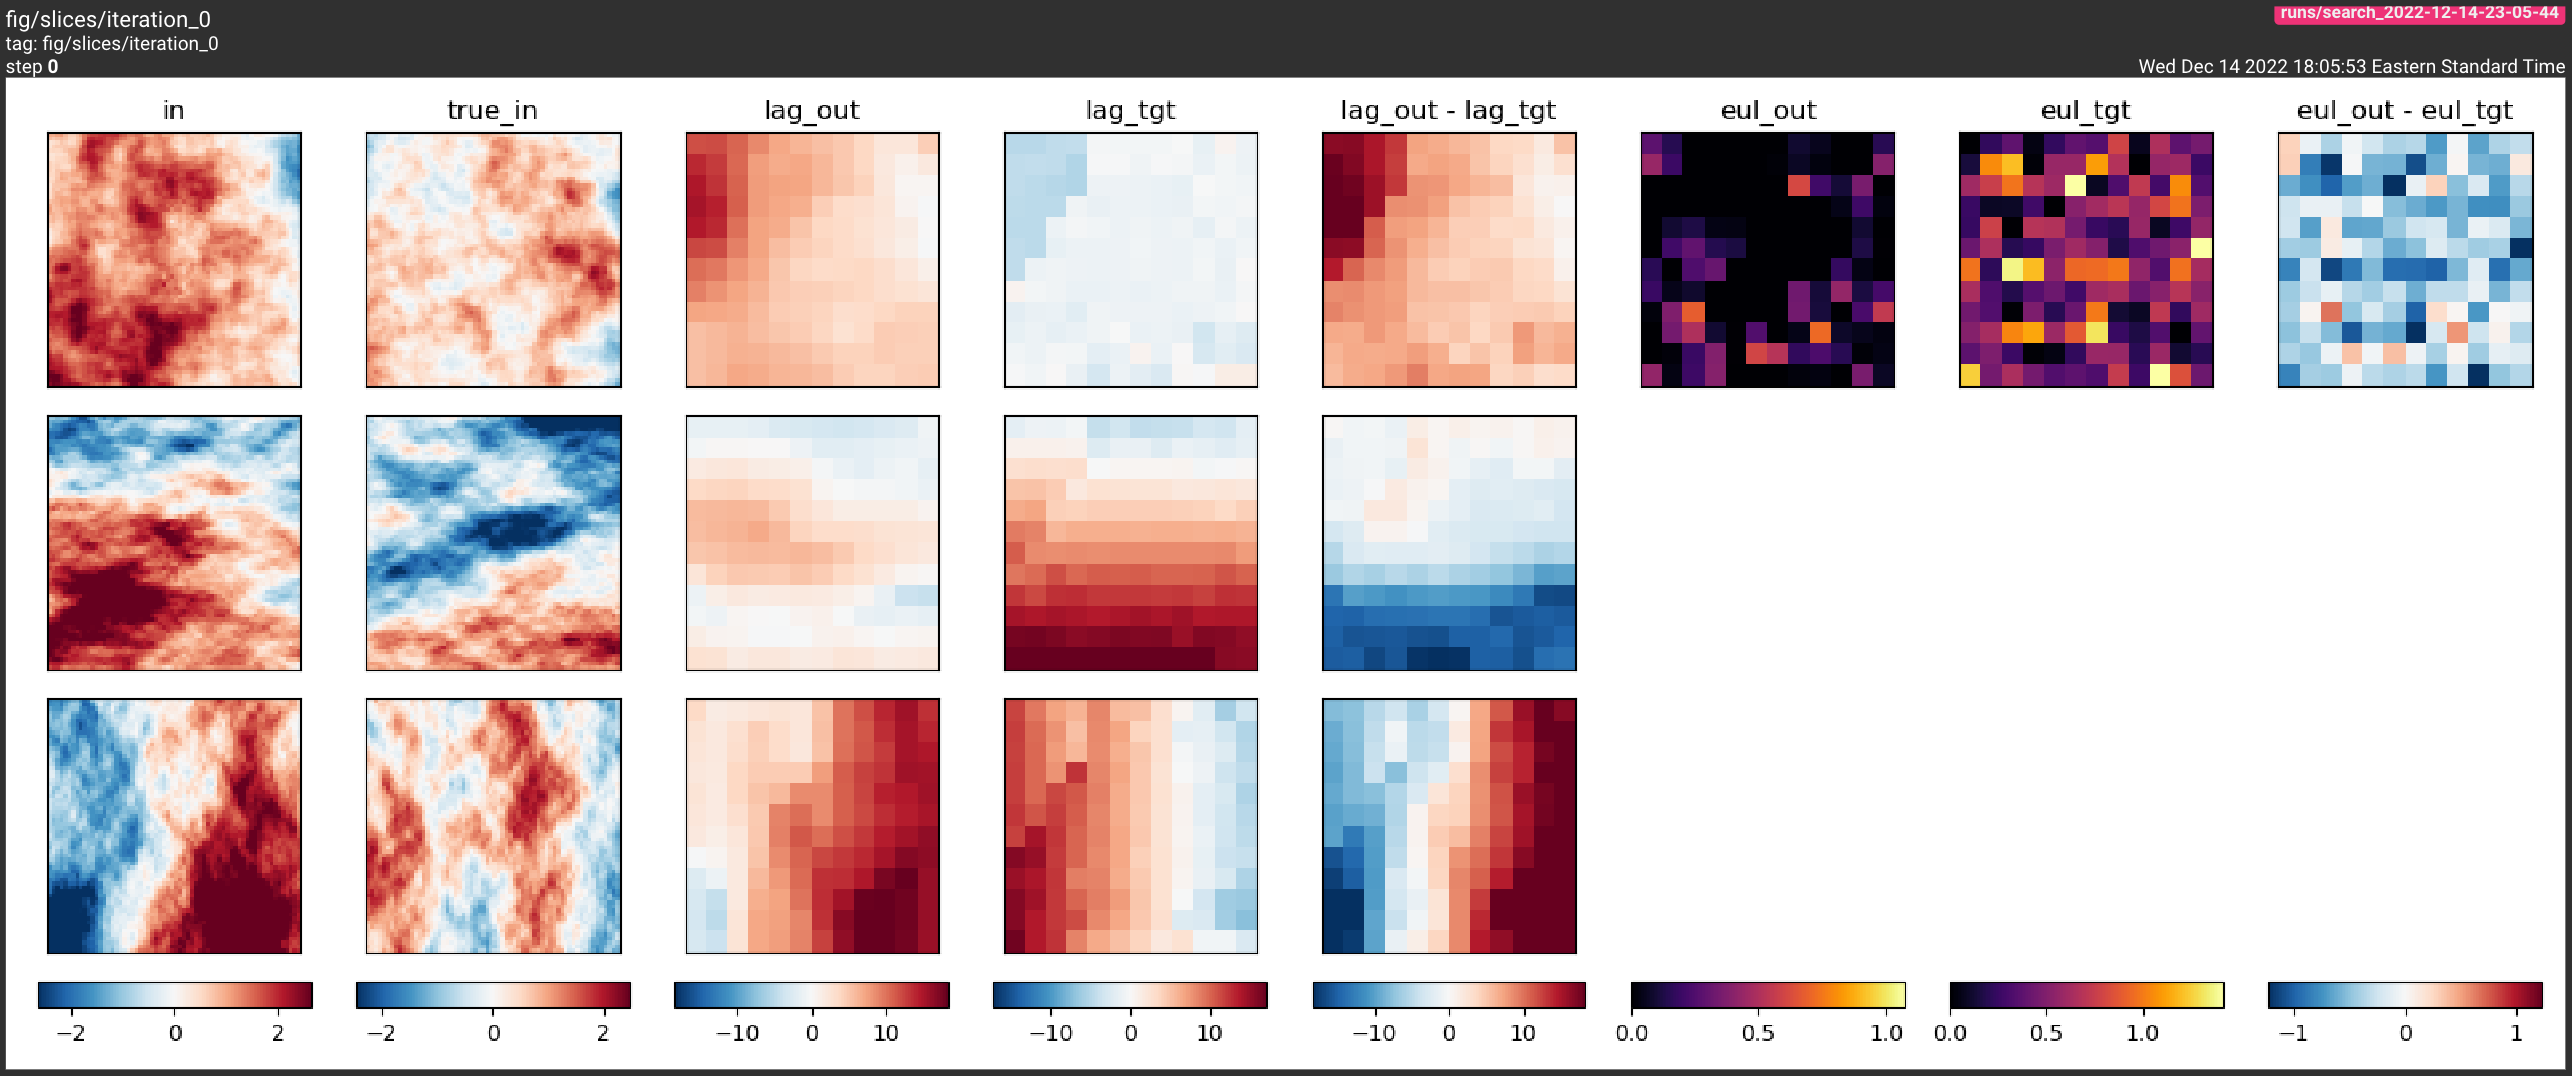
\includegraphics[width=16cm]{figs/initial-displacements.png}
    \caption{The \texttt{in} column displays a slice of the initial linear input field (which was initialized to a patch of the ground truth linear displacement field). The \texttt{true\_in} column displays the ground truth linear input field that we hope to converge to, i.e. it is the answer of our search problem. The other columns show the Lagragian and Eulerian of the forward model output generated from our initial input linear field.}
    \label{fig:init-slices}
\end{figure}

\begin{figure}[h]
    \centering
    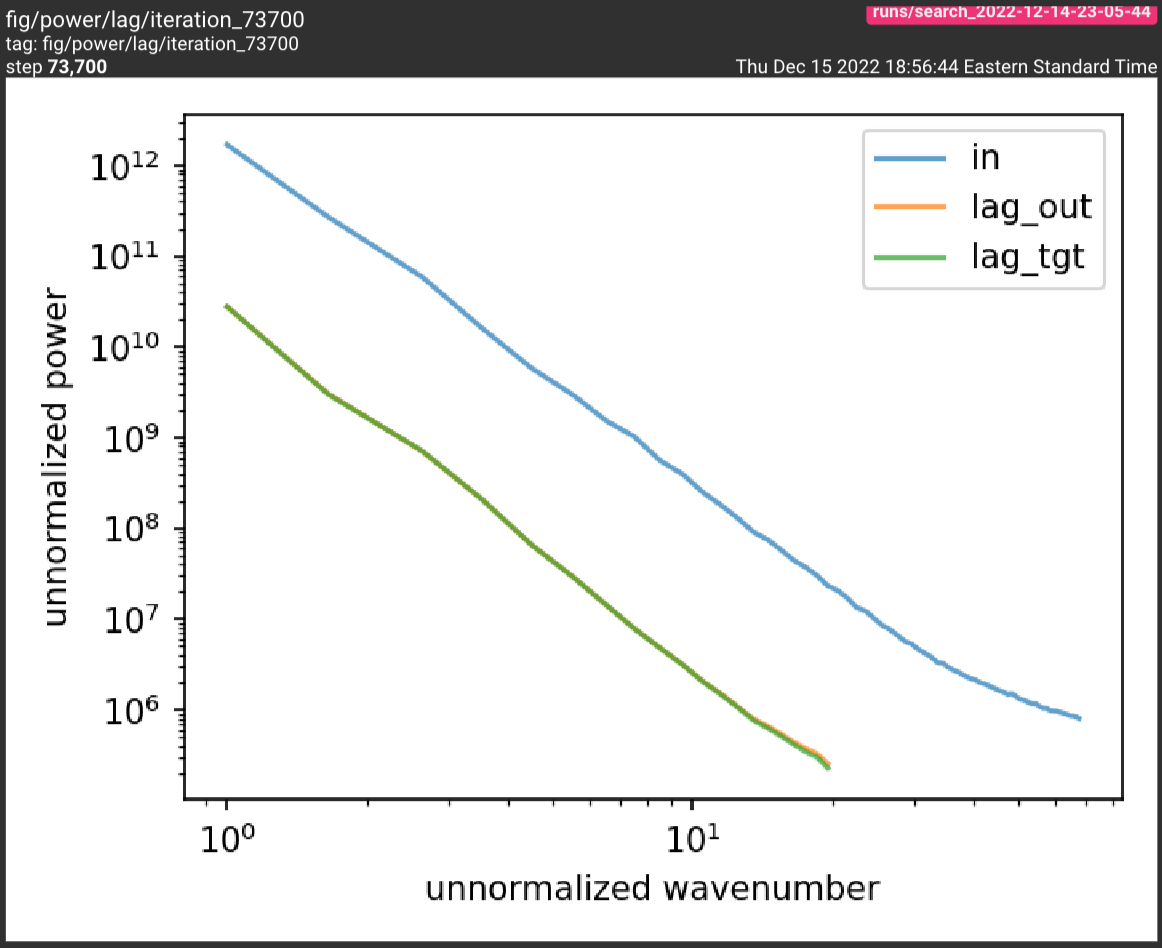
\includegraphics[width=10cm]{figs/final-lag-pow-spec.png}
    \caption{This shows the Lagrangian power spectrum for the linear field learned by gradient descent (after 24 hours)}
    \label{fig:final-lag-pow}
\end{figure}

\begin{figure}[h]
    \centering
    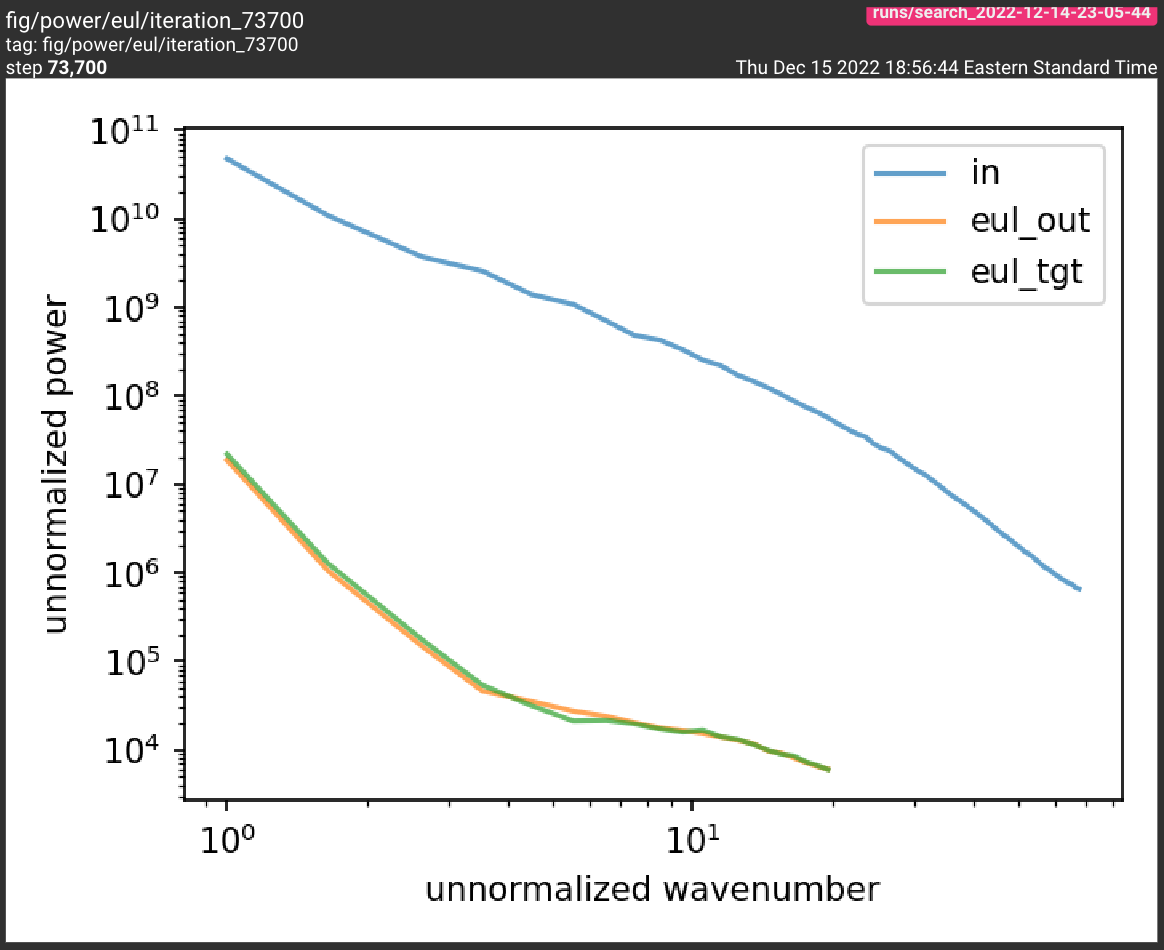
\includegraphics[width=10cm]{figs/final-eul-pow-spec.png}
    \caption{This shows the Eulerian power spectrum for the linear field learned by gradient descent (after 24 hours)}
    \label{fig:final-eul-pow}
\end{figure}

\begin{figure}[h]
    \centering
    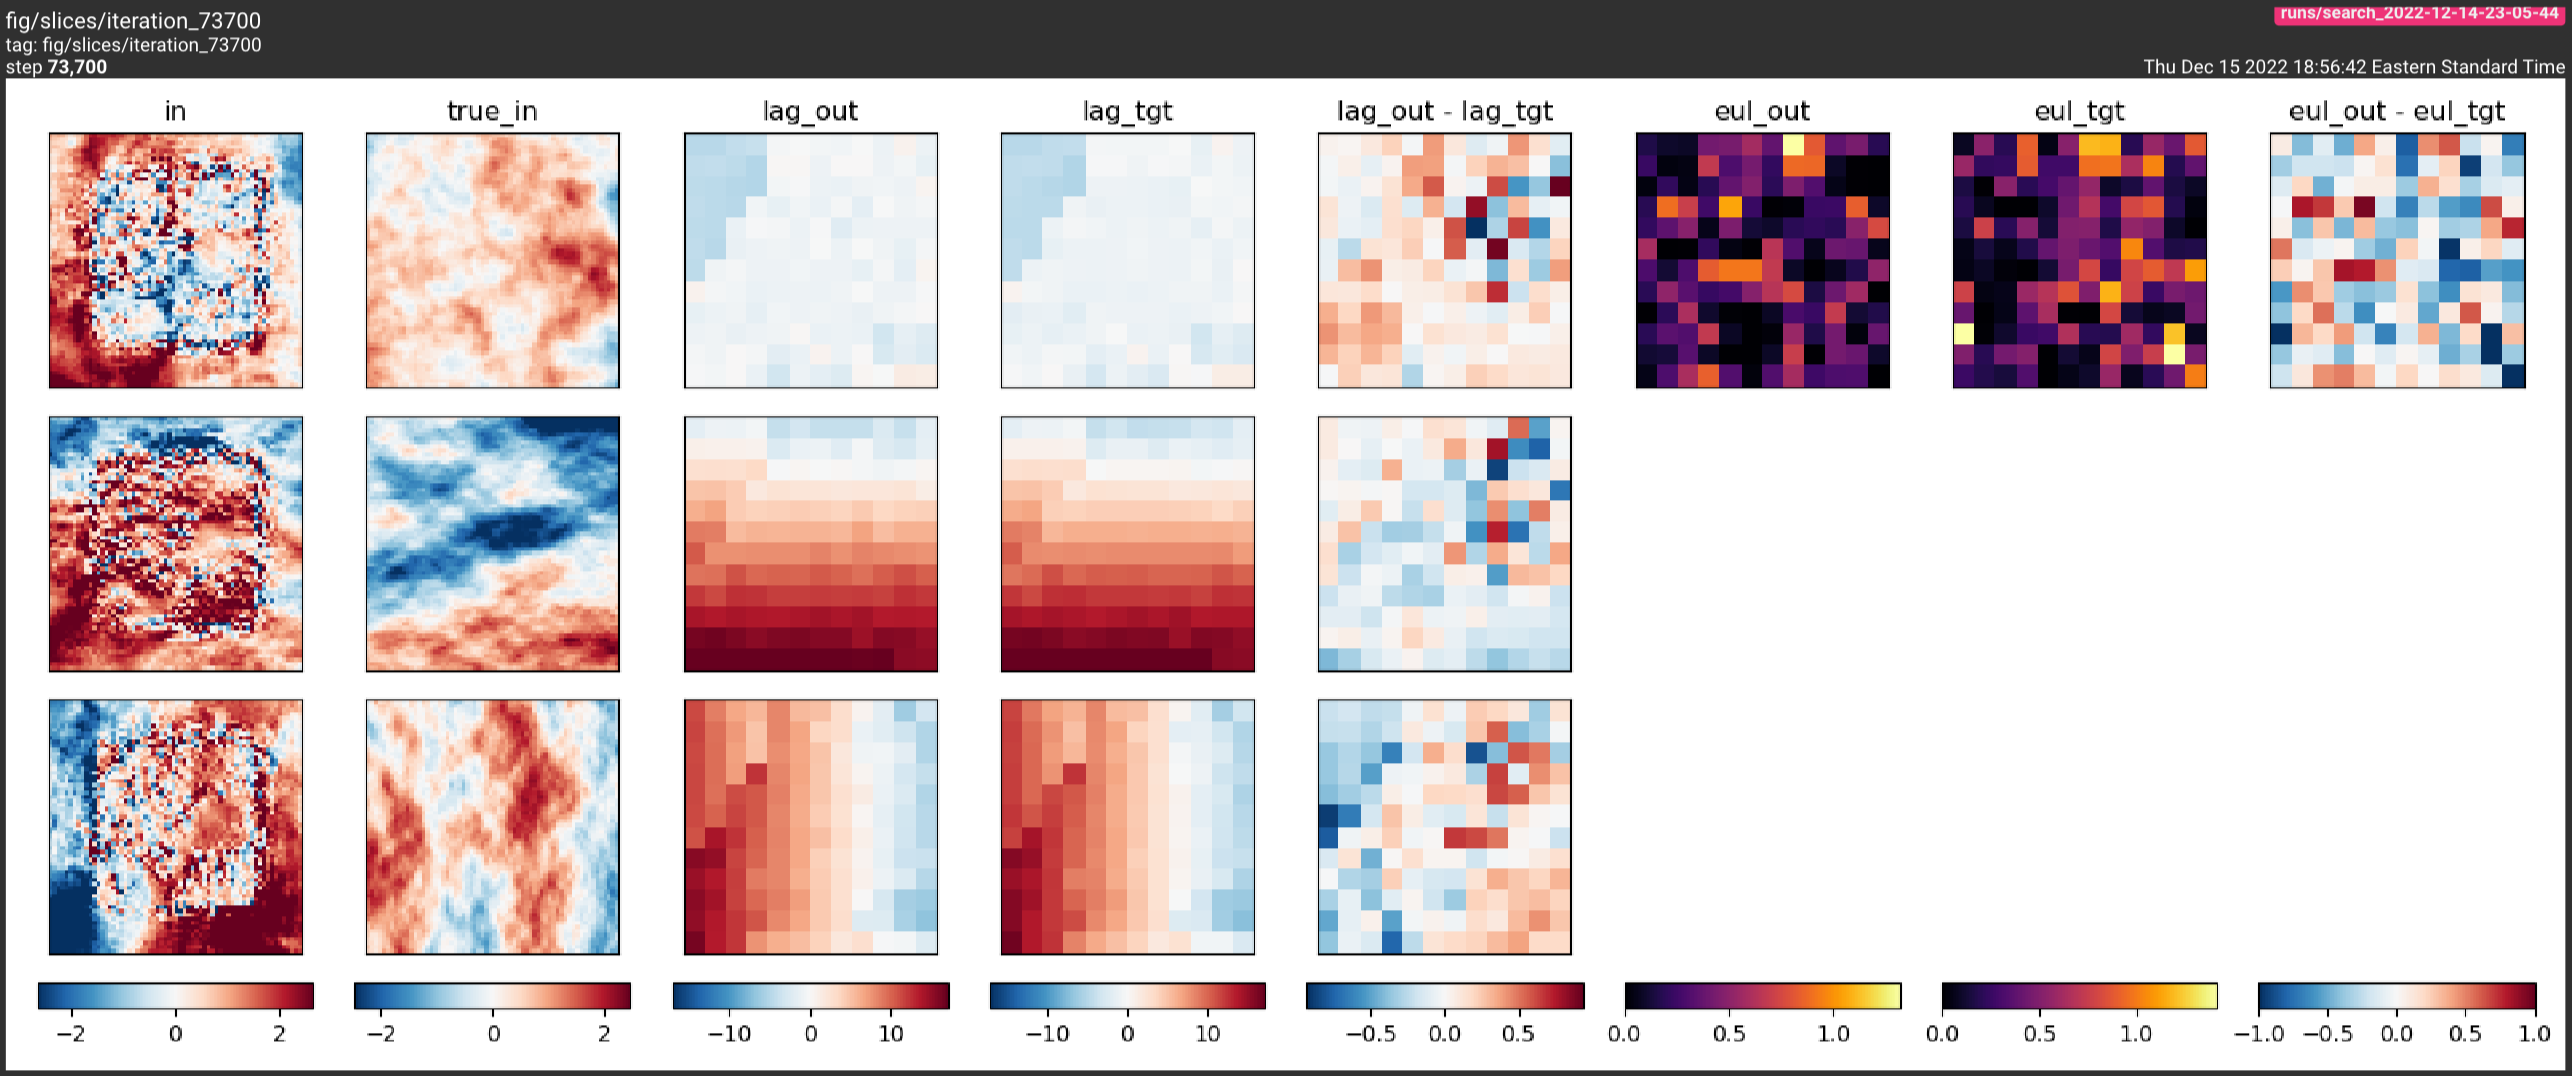
\includegraphics[width=16cm]{figs/final-displacements.png}
    \caption{The \texttt{in} column shows a slice the input linear field learned by gradient descent after 24 hours. The \texttt{true\_in} column displays the ground truth linear input field that we hope to converge to, i.e. it is the answer of our search problem. The other columns show the Lagragian and Eulerian of the forward model output generated from the input linear field learned by the gradient descent.}
    \label{fig:final-slices}
\end{figure}

\clearpage

\subsubsection{Analysis of the plots}

As we can see in Figure \ref{fig:final-lag-pow} and \ref{fig:final-eul-pow}, the input learned by the gradient descent is able to successfully produce a forward model output that matches fairly well with the ground truth in both the Lagrangian and the Eulerian. We can also see this in Figure \ref{fig:final-slices}, where \texttt{lag\_out} (i.e. the Lagrangian of the forward model output) and \texttt{lag\_tgt} (i.e. the Lagrangian of the ground truth) have almost no visible difference.

However, a big problem is that the input displacement field learned by gradient descent seems to show patterns that do not "look like" a cosmology (I am not sure what is the right physics terminology for this). As we can see in Figure \ref{fig:final-slices}, the gradient descent converged to an input that seems to have a ``blur" in the middle, which probably doesn't make sense physically for a cosmology.

\textbf{My guess for why this "blur" occurred}:

Intuitively, I am guessing the reason why this "blur" occurred is that there is nothing in our loss function $\mbox{loss}(\hat{Y}, Y)$ that penalizes the input linear field for not following the structural patterns of a cosmology (i.e. there's nothing in the loss that penalizes the input linear field for being physically non-sense). As a result, the search space for the gradient descent is all possible $40 \times 40 \times 40$ fields, which is too broad. Ideally, we want to constrain the search space to only contain the $40 \times 40 \times 40$ fields that "resembles" a cosmology.

If this is true, then one way to solve this "blur" problem is to add some additional terms in our loss function that penalizes the "structure" of the input field, forcing it to "look like" a cosmology. However, I am not sure if there is any metrics in physics that quantify the degree to which a field "looks like" a cosmology. This might be a question for Shirley.

\clearpage
\bibliography{references}{}
\bibliographystyle{plain}

\end{document}
